\documentclass[tikz,dvipdfmx,dvipsnames]{standalone}

\usepackage{amsmath, amssymb, amsthm, mathrsfs, amsfonts, dsfont}
\usepackage{bbm}
\usepackage{bm}
\usepackage{physics}
\usepackage{ifthen}
\usepackage{setspace}
\usepackage{mathtools}
\usepackage{svg}

\newcommand{\defeq}{\coloneqq}

\newcommand{\red}[1]{\textcolor{red}{#1}}
\newcommand{\blue}[1]{\textcolor{blue}{#1}}
\newcommand{\cyan}[1]{\textcolor{cyan}{#1}}
\newcommand{\gray}[1]{\textcolor{gray}{#1}}
\newcommand{\green}[1]{\textcolor{green}{#1}}
\newcommand{\brown}[1]{\textcolor{brown}{#1}}
\newcommand{\black}[1]{\textcolor{black}{#1}}
\newcommand{\orange}[1]{\textcolor{orange}{#1}}
\newcommand{\purple}[1]{\textcolor{purple}{#1}}
\newcommand{\yellow}[1]{\textcolor{yellow}{#1}}
\newcommand{\Magenta}[1]{\textcolor{Magenta}{#1}}
\newcommand{\RoyalBlue}[1]{\textcolor{RoyalBlue}{#1}}
\newcommand{\RubineRed}[1]{\textcolor{RubineRed}{#1}}
\newcommand{\ForestGreen}[1]{\textcolor{ForestGreen}{#1}}
\newcommand{\YellowOrange}[1]{\textcolor{YellowOrange}{#1}}
\newcommand{\WildStrawberry}[1]{\textcolor{WildStrawberry}{#1}}

\usetikzlibrary{calc,matrix,math}
\usetikzlibrary{decorations.pathreplacing,calligraphy,shapes.arrows}

\usetikzlibrary{
  3d,
  calc,
  math,
  matrix,
  patterns,
  backgrounds,
  arrows.meta,
  shapes.geometric
}


\definecolor{c0}{RGB}{253, 231, 36}
\definecolor{c1}{RGB}{154, 216, 60}
\definecolor{c2}{RGB}{91, 200, 98}
\definecolor{c3}{RGB}{59, 81, 138}
\definecolor{c4}{RGB}{69, 50, 127}

\definecolor{cA}{HTML}{0072BD}
\definecolor{cB}{HTML}{EDB120}
\definecolor{cC}{HTML}{77AC30}
\definecolor{cD}{HTML}{D95319}

\begin{document}

\begin{tikzpicture}
  \node[inner sep=0pt] at (0,0)
  {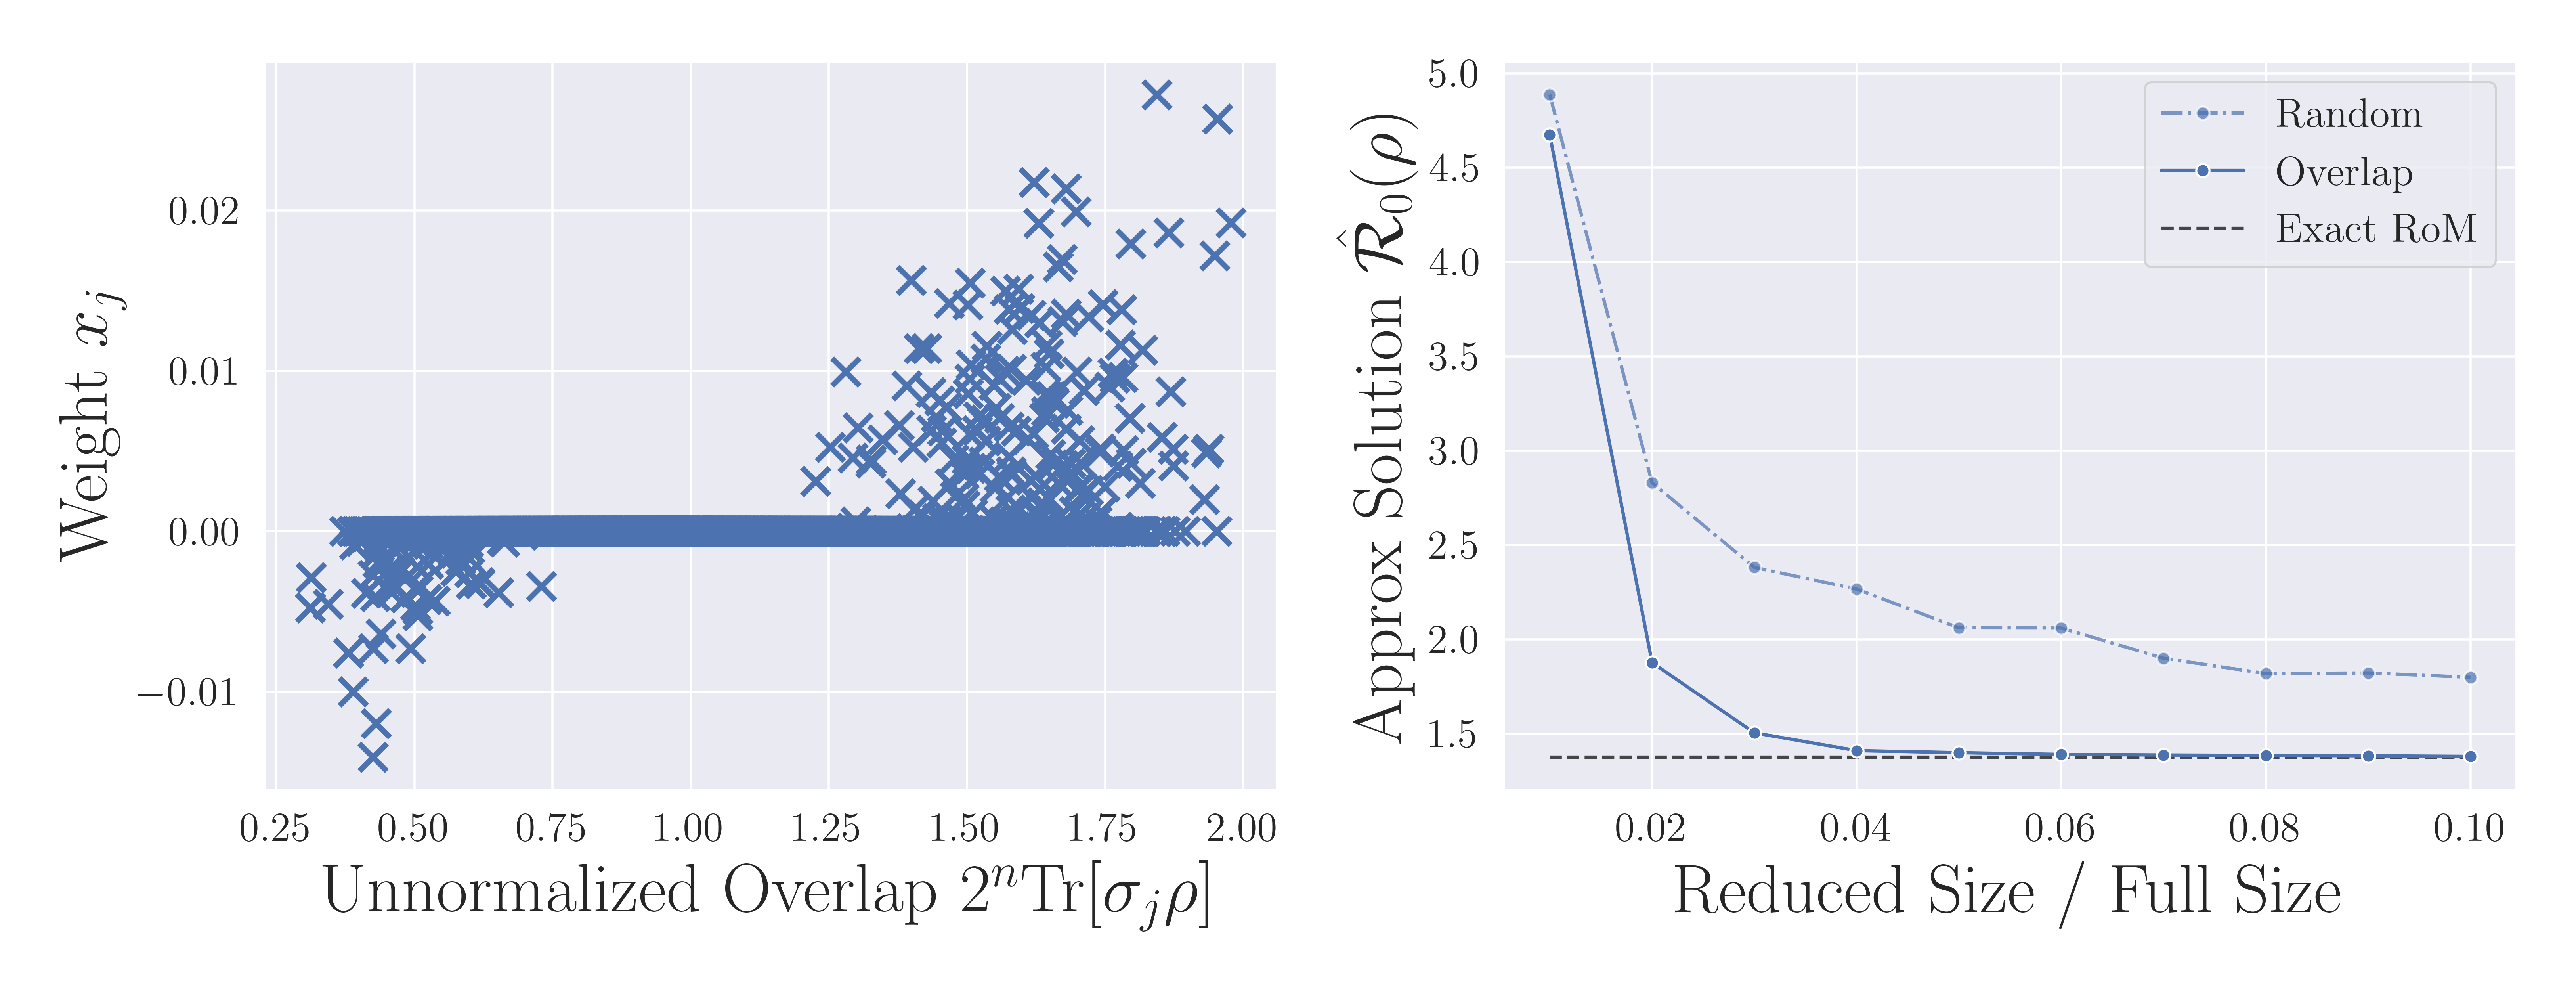
\includegraphics[width=\linewidth]{dot_and_coeff_and_RoM_dot_combined.png}};

  \draw[cD,very thick, rounded corners=0.3cm] (-2.4,-0.1) rectangle (-0.1,2);
  \draw[cA,very thick, rounded corners=0.3cm] (-4.8,-1.3) rectangle (-3.4,-0.25);
  \node[left, align=center] at (-2.5, 1.0) {Contributing\\States\\\small{(non-zero}\\ \small{weights)}};

  \node[cD] at (-1.2, -0.5) {\large{$\rho_+$}};
  \node[cA] at (-3.1, -0.7)  {\large{$\rho_-$}};

  \draw[cC,very thick, rounded corners=0.07cm] (2,-1.3) rectangle (5.7,-1.05) node[midway,left=0.1cm, above=1cm, align=center, font=\small, black] {When chosen with overlaps, \\ still good after reduction.};
\end{tikzpicture}

\end{document}
